\documentclass{article}
\usepackage{xspace,graphicx,amsmath,amsthm,amssymb,xcolor}
\usepackage{listings}
\usepackage{wrapfig}
\usepackage{hyperref}

\setlength{\topmargin}{0.1in}
\setlength{\oddsidemargin}{0in}
\setlength{\evensidemargin}{0in}
\setlength{\headheight}{0in}
\setlength{\headsep}{0in}
\setlength{\textheight}{9in}
\setlength{\textwidth}{6.5in}
\newenvironment{Question}[2][Question]{\begin{trivlist}
\item[\hskip \labelsep {\bfseries #1}\hskip \labelsep {\bfseries #2.}]}{\end{trivlist}}
\title{CS531 Programming assignment \#2}
\author{Matt Meyn, Durga Harish, and Jon Dodge}


\begin{document}
\maketitle
\section{Abstract}

Goal based agents use a search algorithm to find a path to the goal state.  The current problem we are trying to solve fits into the search framework (defined goal, deterministic, known environment, atomic representation of states) .   We explore two different heuristic search algorithms and compare their performance for different initial state. In Particular we present the results using informed search algorithms (A*, Beam Search).  Each of these two algorithms are tested with admissible and inadmissible heuristics functions.

\section{Introduction}

Informed search strategies can outperform uninformed strategies such as breadth-first search by selecting actions to pursue based on an evaluation function. The evaluation function specifies the expected cost of the best path going through that node. Since it is generally not possible to evaluate the cost of a path in advance, this evaluation function is usually an estimate or heuristic.

Our goal in this project is to find useful heuristic functions (both admissible and inadmissible) for a variation on the Towers of Hanoi. Our problem, called Towers of Corvallis, is like the original game except that any disc can be placed on any other, regardless of size. In this problem, the goal is always to reach the state in which all discs are on the first of the three pegs, with the lowest-numbered disc at the bottom, the rest of the discs in ascending order up to the largest number at the top.

We use A* and Beam Search with beam widths 5, 10, 15, 20, 25, 50 and 100. Each of these searches is performed with four different heuristic functions, two admissible and two inadmissible.


\section{Algorithms-Heuristic Functions}
We tested two functions as heuristics: one admissible and one inadmissible.\\


\textbf{Heuristic Function 1 }considers the first disc on Peg A that isout of solution order. The function adds the number of discs above to the total cost of this state. This is the minimum possible actual cost of a solution path through this state, because at least one move is needed to move each disc above the “bad” disc to another peg, and at least one more move to move the “bad” disc.  For the other two pegs, the desired order is in reverse so that the discs can be easily placed on Peg A when possible. All discs out of desired order on Pegs B and C are assigned a cost of 1, because at least one move will be necessary to move them to Peg A.

\begin{lstlisting}[frame=single]

NumDiscsOutOfPlaceAllPegs( SearchState ) returns Cost
	Cost <- 0
	PegA <- SearchState.Pegs[1]
	for each Disc in PegA reverse order
		DiscsAbove <- PegANum Discs - Disc.Position
		DesiredDiscValue <- MAX_DISC_VALUE - Disc.Position
		if Disc.Value != DesiredDiscValue
			Cost <- DiscsAbove

	for each remaining Peg
		for each Disc in Peg
			if Disc.Value != Disc.Position
  				Cost <- Cost + 1	
return Cost

\end{lstlisting}

\begin{lstlisting}[frame=single]

ManhattanDistanceAllPeg( SearchState )
	Cost <- 0
	PegA <- SearchState.FirstPeg
	IsInOrder <- True
	for each Disc in PegA
		DesiredDiscValue <- MAX_DISC_SIZE - Disc.Position
		IsInOrder <- IsInOrder AND PegA == DesiredDiscValue
		if NOT IsInOrder
			Cost <- Cost + 2 + Abs( Disc.Value - DesiredDiscValue )

	for each remaining Peg
		for each Disc in Peg
			Cost <- Cost + 1
			for each OtherDisc above Disc 
				delta <- Disc.Value - OtherDisc.Value
				if delta > 0
					Cost <- Cost + delta
	
	return Cost


\end{lstlisting}

\begin{figure}[h!]
\centering
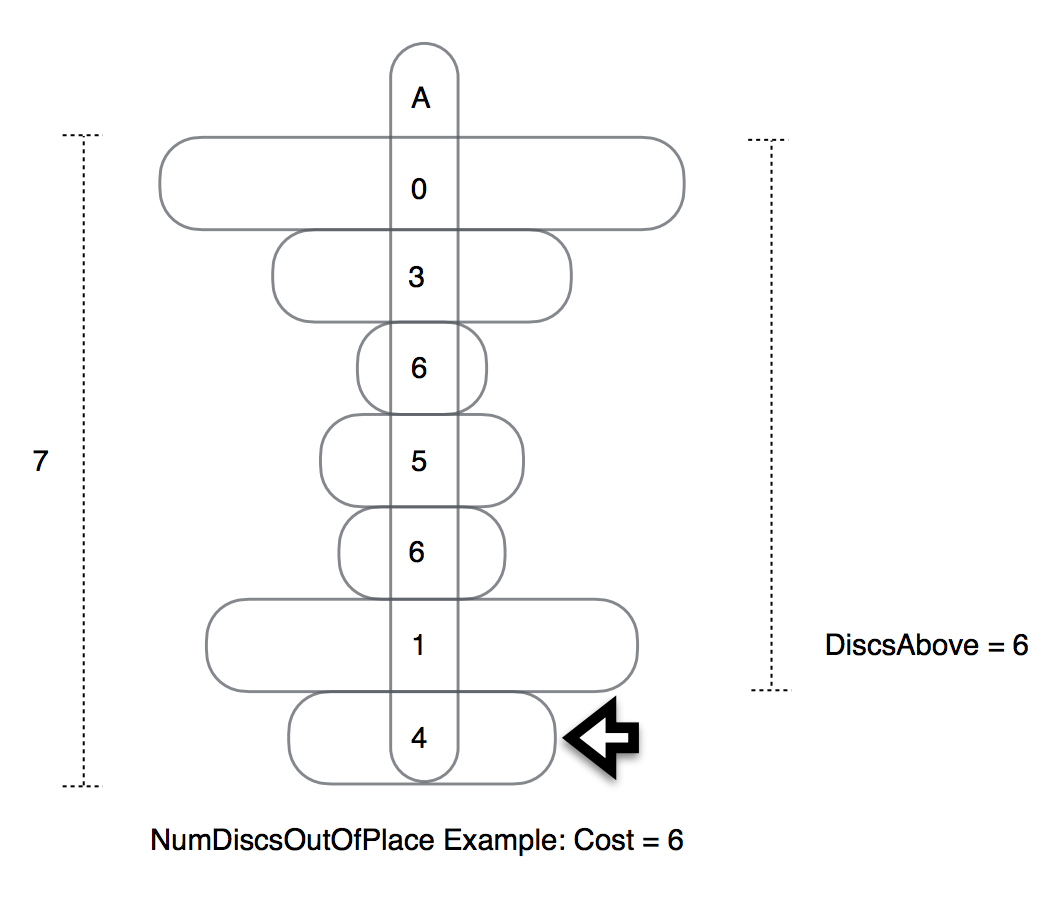
\includegraphics[width=0.7\linewidth]{Diagram1.png}
\caption{FIXME with Content}
\label{fig:reflex}
\end{figure}

\begin{figure}[h!]
\centering
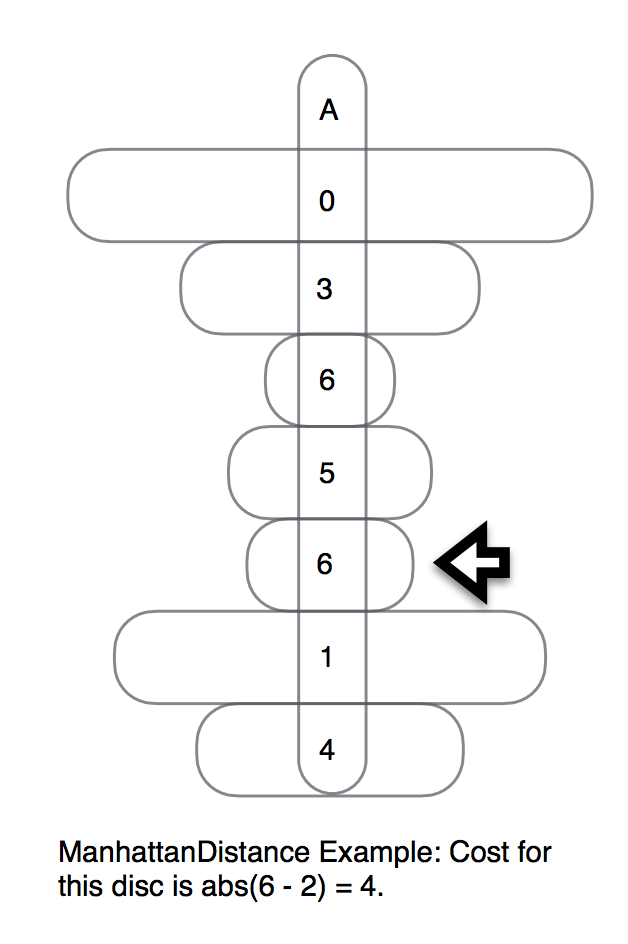
\includegraphics[width=0.7\linewidth]{Diagram2.png}
\caption{FIXME with Content}
\label{fig:reflex}
\end{figure}

\section{Results}
 we carried out the experiment with two search algorithms(A-Star, Beam Search).  As mentioned previously, we used two heuristic functions one admissible and one in-admissible.  Fig1, Fig2, Fig3 show the plots of number of nodes expanded, CPU Clock time in log-scale, Depth of the search tree w.r.t to problem size. 



\begin{table}[h!]
\centering
\caption{Table showing the results for A-Star search algorithm. Failures column indicate number of times the function failed.}
\label{my-label}
\begin{tabular}{|l|l|l|l|l|l|}
\hline
\textbf{Heuristic Function} & \textbf{Problem Size} & \textbf{Failures} & \textbf{Solution Depth} & \textbf{Nodes Expanded} & \textbf{CPU Time} \\ \hline
In Admissible               & 3                     & 0                 & 5                           & 6                           & 0.00282839999995        \\ \hline
In Admissible               & 4                     & 0                 & 7                           & 8                           & 0.00612550000004        \\ \hline
In Admissible               & 5                     & 0                 & 11                          & 12                          & 0.01271615              \\ \hline
In Admissible               & 6                     & 0                 & 14                          & 16                          & ,0.0214712              \\ \hline
In Admissible               & 7                     & 0                 & 16                          & 18                          & 0.0295876               \\ \hline
In Admissible               & 8                     & 0                 & 19                          & 25                          & 0.05099955              \\ \hline
In Admissible               & 9                     & 0                 & 23                          & 31                          & 0.0776069               \\ \hline
In Admissible               & 10                    & 0                 & 26                          & 40                          & 0.1196321               \\ \hline
Admissible                  & 3                     & 0                 & 5                           & 15                          & 0.00789120000004,       \\ \hline
Admissible                  & 4                     & 0                 & 7                           & 57                          & 0.054209                \\ \hline
Admissible                  & 5                     & 6                 & 7                           & 163                         & 0.3248069               \\ \hline
Admissible                  & 6                     & 18                & 1                           & 29                          & 0.08015595              \\ \hline
\end{tabular}
\end{table}



\begin{figure}[h!]
\centering
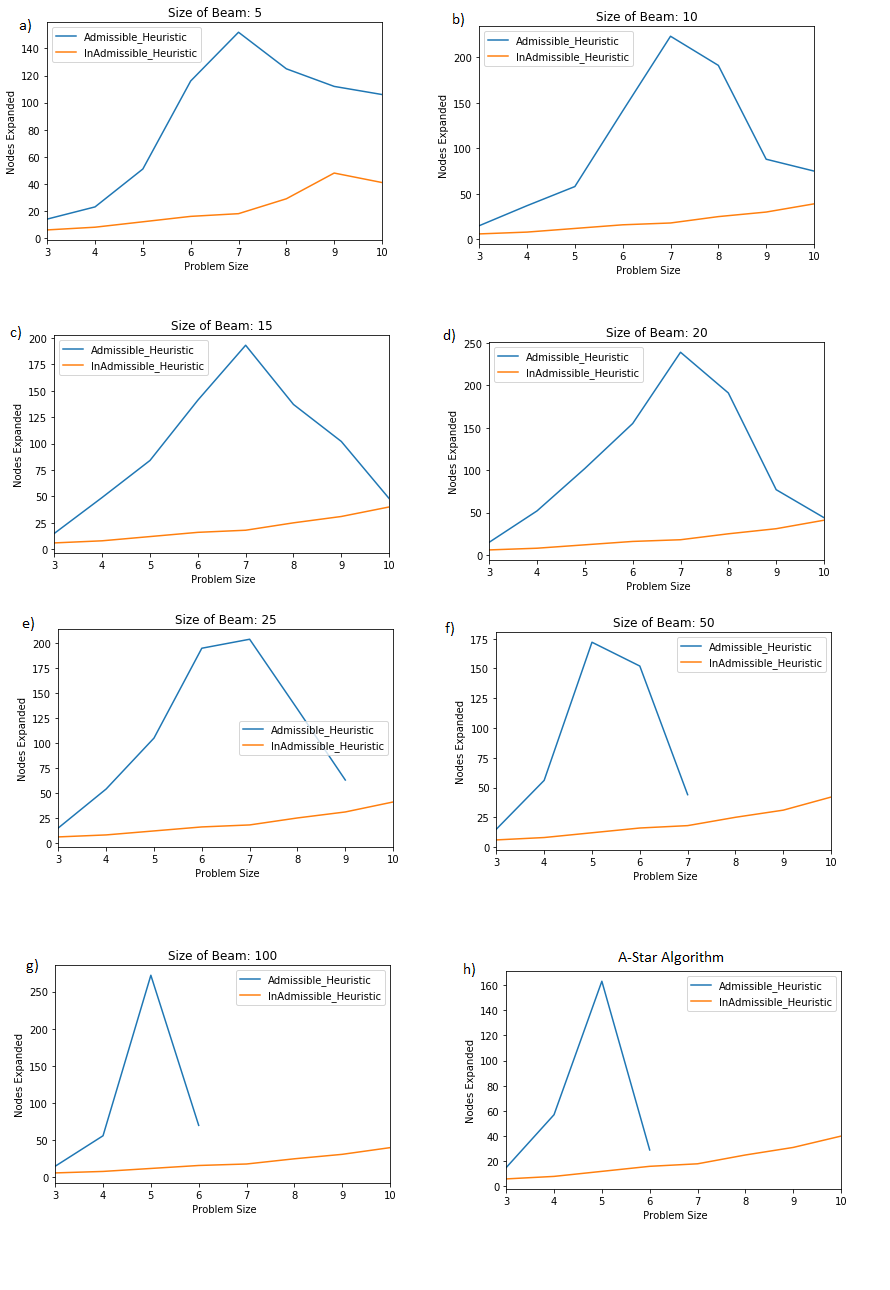
\includegraphics[width=0.7\linewidth]{all_nodes_expanded.png}
\caption{FIXME with Content}
\label{fig:reflex}
\end{figure}


\begin{figure}[h!]
\centering
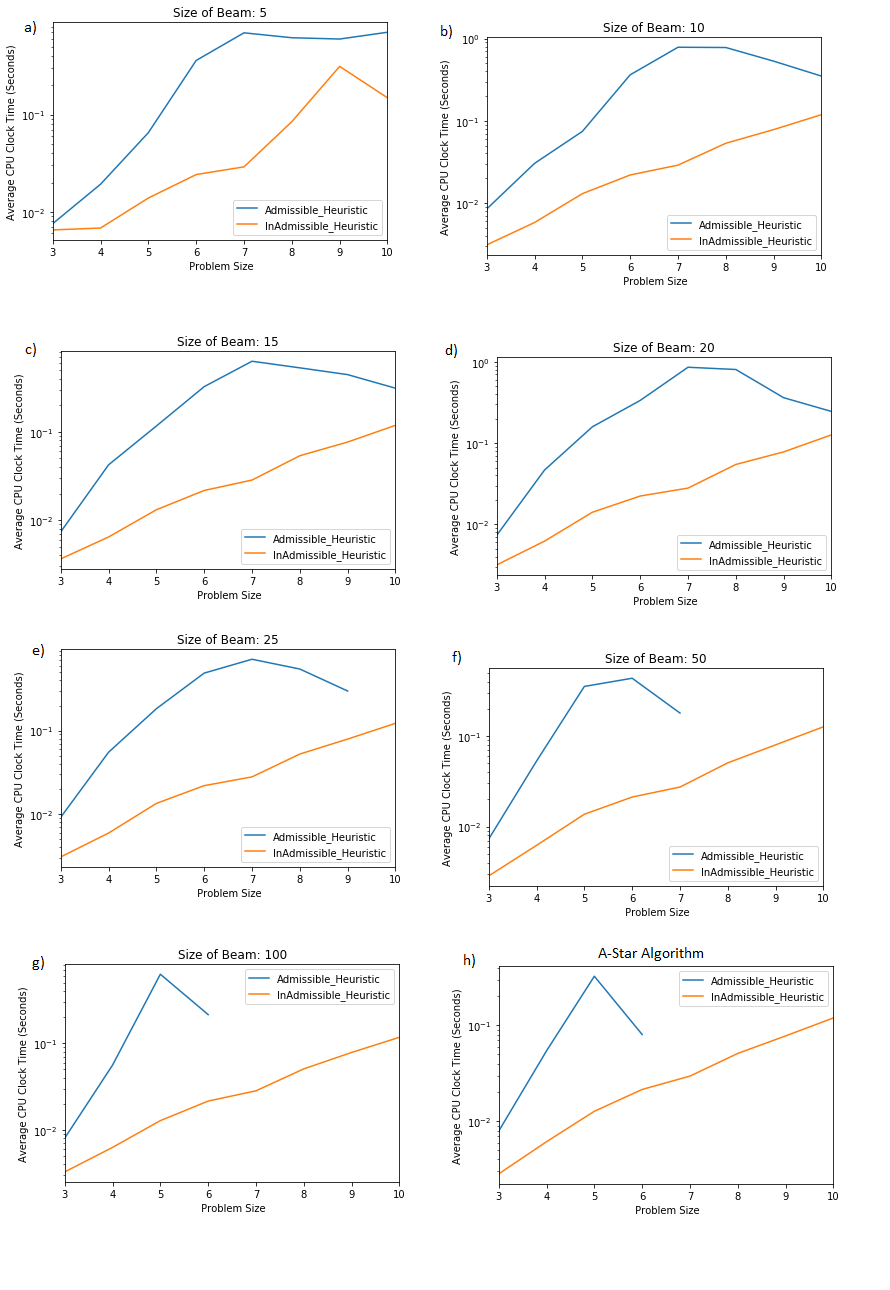
\includegraphics[width=0.7\linewidth]{cpu_time_all.png}
\caption{FIXME with Content}
\label{fig:reflex}
\end{figure}


\begin{figure}[h!]
\centering
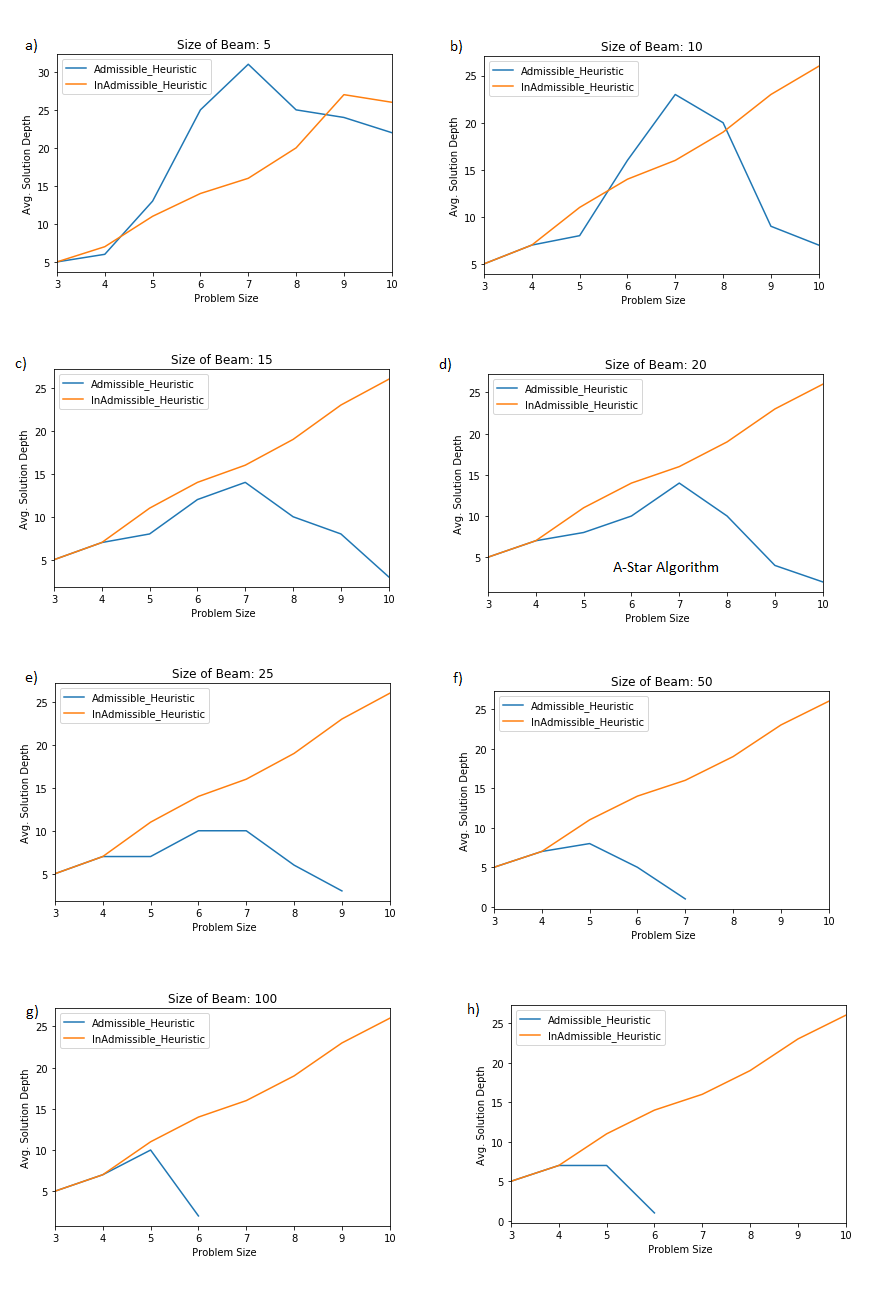
\includegraphics[width=0.7\linewidth]{all_solution_depth.png}
\caption{FIXME with Content}
\label{fig:reflex}
\end{figure}

\section{Discussion}


%%%%%%%%%%%%%%%%%%%%%%%%%%%%%%%%%%%%%%%%%%%%%%%%%%%%%%%%%%%%%%%%%%%%%%%%%%%%%%%%%%%%%%%%%%%%%%%%%%%%%%%%%%
\begin{Question}{1}Show an example solution sequence for each algorithm for the largest size you tested in the following format:
We tested for disc size of 10 and peg size of 3. 


\end{Question}


%%%%%%%%%%%%%%%%%%%%%%%%%%%%%%%%%%%%%%%%%%%%%%%%%%%%%%%%%%%%%%%%%%%%%%%%%%%%%%%%%%%%%%%%%%%%%%%%%%%%%%%%%%
%%%%%%%%%%%%%%%%%%%%%%%%%%%%%%%%%%%%%%%%%%%%%%%%%%%%%%%%%%%%%%%%%%%%%%%%%%%%%%%%%%%%%%%%%%%%%%%%%%%%%%%%%%

\begin{Question}{2}How did the search time and the solution quality vary with the beam width? Is there a beam width that gives the best tradeoff for the two heuristics?

Up to a beam width of about 20, the search time increased only modestly. At 20 it increased significantly. With the inadmissible heuristic, the solution quality did not vary, but with the admissible heuristic, there was some improvement of solution quality as beam width increased.

\end{Question}

%%%%%%%%%%%%%%%%%%%%%%%%%%%%%%%%%%%%%%%%%%%%%%%%%%%%%%%%%%%%%%%%%%%%%%%%%%%%%%%%%%%%%%%%%%%%%%%%%%%%%%%%%%
%%%%%%%%%%%%%%%%%%%%%%%%%%%%%%%%%%%%%%%%%%%%%%%%%%%%%%%%%%%%%%%%%%%%%%%%%%%%%%%%%%%%%%%%%%%%%%%%%%%%%%%%%%

\begin{Question}{3} Is there a clear preference ordering among the heuristics you tested considering the number of nodes searched and the total CPU time taken to solve the problems for the two algorithms?

With respect to both the number of nodes searched and the total CPU time needed, our inadmissible heuristic substantially outperformed our admissible heuristic. 

The number of nodes expanded by A* and beam search (all beam sizes) using the admissible heuristic appear to have complexity exponential in the problem size. For the same beam widths, A* and beam search using the inadmissible heuristic show approximately linear complexity.

The CPU time required to find a solution shows a less dramatic but still apparent difference in time complexity. 

\end{Question}

%%%%%%%%%%%%%%%%%%%%%%%%%%%%%%%%%%%%%%%%%%%%%%%%%%%%%%%%%%%%%%%%%%%%%%%%%%%%%%%%%%%%%%%%%%%%%%%%%%%%%%%%%%
%%%%%%%%%%%%%%%%%%%%%%%%%%%%%%%%%%%%%%%%%%%%%%%%%%%%%%%%%%%%%%%%%%%%%%%%%%%%%%%%%%%%%%%%%%%%%%%%%%%%%%%%%%

\begin{Question}{4}Can a small sacrifice in optimality give a large reduction in the number of nodes expanded? What about CPU time?
A* tree search using an admissible heuristic guarantees an optimal solution, but this guarantee comes at a cost. The requirement of admissibility imposes constraints on the choices we can make for how to estimate the cost of a given state. It is clearly easier to find heuristics that lead more quickly to a goal state if those constraints are removed.

As observed above in (3), our inadmissible heuristic function enabled all searches to expand a number of nodes approximately linear in the problem size, whereas the complexity associated with the admissible heuristic appears to be exponential. 

\end{Question}

%%%%%%%%%%%%%%%%%%%%%%%%%%%%%%%%%%%%%%%%%%%%%%%%%%%%%%%%%%%%%%%%%%%%%%%%%%%%%%%%%%%%%%%%%%%%%%%%%%%%%%%%%%
%%%%%%%%%%%%%%%%%%%%%%%%%%%%%%%%%%%%%%%%%%%%%%%%%%%%%%%%%%%%%%%%%%%%%%%%%%%%%%%%%%%%%%%%%%%%%%%%%%%%%%%%%%
\begin{Question}{5}How did you come up with your heuristic evaluation functions?
Our admissible heuristic function, Function 1, is based on the simplified problem that if a disc on Peg A is out of solution order, every disc above it must be moved. Similarly, every disc on Pegs B and C that is not sorted in reverse order also represents an extra move to get that disc out of the way.

Function 2, our inadmissible heuristic, was inspired by the “Manhattan Distance” heuristic. Each disc on Peg A from position 0 up that is in order is already at the “destination.” After a disc is found out of order, each disc incurs an extra cost of the absolute value of the delta between the desired disc “size” and actual disc “size.” This lets our search algorithm know that if Peg A is “approximately” in order, this is closer to the solution. 

On the other pegs, we decided to sum the deltas in “size” between each disc and each lower-numbered disc above it, adding the sum of all of these to the total cost, because states with Pegs B and C stacked in ascending order from bottom to top should be favored.


\end{Question}


%%%%%%%%%%%%%%%%%%%%%%%%%%%%%%%%%%%%%%%%%%%%%%%%%%%%%%%%%%%%%%%%%%%%%%%%%%%%%%%%%%%%%%%%%%%%%%%%%%%%%%%%%%
%%%%%%%%%%%%%%%%%%%%%%%%%%%%%%%%%%%%%%%%%%%%%%%%%%%%%%%%%%%%%%%%%%%%%%%%%%%%%%%%%%%%%%%%%%%%%%%%%%%%%%%%%%

\begin{Question}{6} How do the two algorithms compare in the amount of search involved and the cpu-time
The two algorithms, A* and Beam Search, are related in that A* is Beam Search with a beam of unbounded width. Naturally, then, A* does expand more nodes and take more time than a beam search with width, say, 15. But when comparing to a beam width of 100, there does not seem to be a significant difference for this problem.

\end{Question}

%%%%%%%%%%%%%%%%%%%%%%%%%%%%%%%%%%%%%%%%%%%%%%%%%%%%%%%%%%%%%%%%%%%%%%%%%%%%%%%%%%%%%%%%%%%%%%%%%%%%%%%%%%
%%%%%%%%%%%%%%%%%%%%%%%%%%%%%%%%%%%%%%%%%%%%%%%%%%%%%%%%%%%%%%%%%%%%%%%%%%%%%%%%%%%%%%%%%%%%%%%%%%%%%%%%%%
\begin{Question}{7}Do you think that either of these algorithms scale to even larger problems? What is the largest problem you could solve with the best algorithm+heuristic combination? Report the wall-clock time, CPU-time, and the number of nodes searched.

Our admissible heuristic would not scale well to larger problems because it increases the number of nodes expanded exponentially. The inadmissible heuristic also is more tractable in terms of CPU time.

The curves for the admissible heuristic also increase more steeply as the beam width increases toward infinite width.



\end{Question}



%%%%%%%%%%%%%%%%%%%%%%%%%%%%%%%%%%%%%%%%%%%%%%%%%%%%%%%%%%%%%%%%%%%%%%%%%%%%%%%%%%%%%%%%%%%%%%%%%%%%%%%%%%
%%%%%%%%%%%%%%%%%%%%%%%%%%%%%%%%%%%%%%%%%%%%%%%%%%%%%%%%%%%%%%%%%%%%%%%%%%%%%%%%%%%%%%%%%%%%%%%%%%%%%%%%%%

\begin{Question}{8}Is there any tradeoff between how good a heuristic is in cutting down the number of nodes and how long it took to compute? Can you quantify it?




\end{Question}

%%%%%%%%%%%%%%%%%%%%%%%%%%%%%%%%%%%%%%%%%%%%%%%%%%%%%%%%%%%%%%%%%%%%%%%%%%%%%%%%%%%%%%%%%%%%%%%%%%%%%%%%%%
%%%%%%%%%%%%%%%%%%%%%%%%%%%%%%%%%%%%%%%%%%%%%%%%%%%%%%%%%%%%%%%%%%%%%%%%%%%%%%%%%%%%%%%%%%%%%%%%%%%%%%%%%%
\begin{Question}{9}Is there anything else you found that is of interest?


\end{Question}

%%%%%%%%%%%%%%%%%%%%%%%%%%%%%%%%%%%%%%%%%%%%%%%%%%%%%%%%%%%%%%%%%%%%%%%%%%%%%%%%%%%%%%%%%%%%%%%%%%%%%%%%%%
%%%%%%%%%%%%%%%%%%%%%%%%%%%%%%%%%%%%%%%%%%%%%%%%%%%%%%%%%%%%%%%%%%%%%%%%%%%%%%%%%%%%%%%%%%%%%%%%%%%%%%%%%%



















\end{document}